\documentclass[a4paper,12pt]{article}

\usepackage[utf8]{inputenc}
\usepackage[ngerman]{babel}
\usepackage{amsmath,amssymb}
\usepackage{graphicx}
\usepackage[a4paper, left=2cm, right=3cm, bottom=2cm]{geometry}
\usepackage{fancyhdr}
\usepackage{qrcode}
\usepackage{hyperref}
\usepackage{breakurl}
\usepackage{imakeidx}
\usepackage{wrapfig}

\graphicspath{ {./images/} }

\title{Die Atombombe}
\author{Tim, Olli, Jakub}
\date{\today}

\begin{document}
\pagestyle{fancy}

\fancyfoot[LE,RO]{\thepage}
\fancyfoot[LO,CE]{Tim, Olli, J. Z.}
\fancyfoot[CO,RE]{Atombombe}

\maketitle

\begin{abstract}
nn
\end{abstract}

\newpage

\tableofcontents

\newpage

\section{Einführiung}
ngerman\cite{ngerman}.

\section{Aufbau}
\begin{wrapfigure}{r}{0.4\textwidth}
    \vspace{-1.4cm}
    \centering
    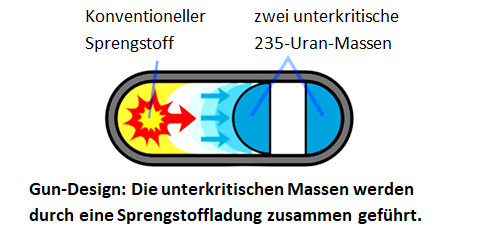
\includegraphics[scale=0.7]{Gun.png}
    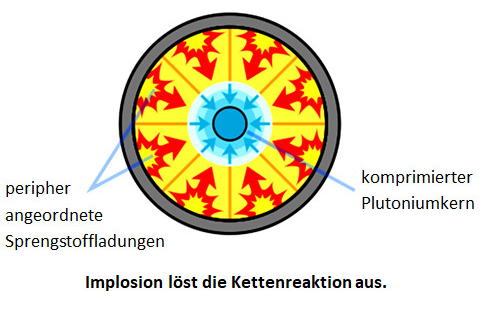
\includegraphics[scale=0.7]{Implosion.png}
\end{wrapfigure}

\textbf{Gun-Design:}
Zwei unterkritische Massen von Uran-235 befinden sich an gegenüberliegenden Enden. 
Konventioneller Sprengstoff (z. B. TNT) befindet sich hinter einer der Massen. \hyperlink{gun_section}{Erklärung gibts auf Seite 4.}

\vspace*{4cm}

\noindent\textbf{Implosions-Design:}
Ein Plutoniumkern liegt im Zentrum. Ringsherum sind konventionelle Sprengladungen 
in einem speziellen Muster (meist sphärisch) angeordnet. \hyperlink{implosion_section}{Erklärung gibts auf Seite 4.}

\newpage

\section{Funktion}
\hypertarget{implosion_section}{}
\hypertarget{gun_section}{}

\newpage

\section{Links}
\begin{center}
\qrcode{https://github.com/Jason4225/Latex}
\end{center}
\bigskip

\href{https://github.com/Tim-foe}{Github: Tim} \hspace{4cm}
\href{https://github.com/YoOlli}{Github: Olli} \hspace{4cm}
\href{https://github.com/Jason4225}{Github: J. Z.}

\bibliographystyle{plain}
\bibliography{bibliography.bib}

\end{document}